% Author Name: José Areia 
% Author Contact: jose.apareia@gmail.com
% Version: 2.2.13 - 2026/01/06
% Public Repository: https://github.com/joseareia/ipleiria-thesis
% Wiki/Getting Help: https://github.com/joseareia/ipleiria-thesis/wiki

%%% Document Options %%%
\documentclass[
    language=english,
    school=hcmus,
    docstage=final,
    media=screen,
    bookprint=false,
    linkcolor=blue!55!black,
    chapterstyle=fancy,
    coverstyle=classic,
    aiacknowledgement=false,
    listprefix=false
]{ReportThesis} % Refer to the Wiki for a list of available options.

%%% Document Version %%%
\DocumentVersion{1.0.0} % Required only if the 'docstage' is set to 'working'.

%%% Document Metadata %%%
% First Author (Mandatory)
\FirstAuthor{Nguyen Do Bao}
\FirstAuthorNumber{23127026}

% Second Author (Optional)
% \SecondAuthor{Jane Smith}
% \SecondAuthorNumber{2230456}

% Third Author (Optional)
% \ThirdAuthor{July Smith}
% \ThirdAuthorNumber{2230457}

% Supervisor (Mandatory)
\Supervisor{Le Nhut Nam, M.Sc.}
\SupervisorMail{}
\SupervisorTitle{Faculty of Information Technology}

% Co-Supervisor (Optional)
\CoSupervisor{Nguyen Ngoc Duc, M.Sc.}
\CoSupervisorMail{}
\CoSupervisorTitle{Faculty of Information Technology}

% Second Co-Supervisor (Optional)
\SecCoSupervisor{Nguyen Thi Thu Hang, M.Sc.}
\SecCoSupervisorMail{}
\SecCoSupervisorTitle{Faculty of Information Technology}

% Title (Mandatory)
\Title{Project 3 - Clustering with Applications}

% Subtitle (Mandatory)
\Subtitle{An Improved Federated Clustering Algorithm with Model-based Clustering}

% University (Mandatory)
\University{Vietnam National University, Ho Chi Minh City}

% School (Mandatory)
\School{University of Science}

% Department (Mandatory)
\Department{Faculty of Information Technology}

% Degree (Mandatory)
\Degree{}

% Course (Optional)
\Course{CSC14004 - Data Mining and Applications}

% Local & Date (Mandatory)
\Date{Ho Chi Minh City, April 2026}

% Academic Year
\AcademicYear{2025/2026}


\begin{document}

%%% Front Matter %%%
\include{Matter/00-Cover}
\include{Matter/01-Front-Page}

%%% Copyright Statement %%%
% \include{Matter/02-Copyright}

%%% Roman Numeration %%%
\pagenumbering{roman}

%%% Acknowledgements %%%
% \include{Matter/03-Acknowledgements}

%%% Abstract %%%
\thispagestyle{plain}

\pdfbookmark[1]{Abstract}{abstract}
\chapter*{Abstract}

This report studies SR-FCA (\textit{Successive Refine Federated Clustering Algorithm}, Vardhan, Ghosh and Mazumdar, TMLR~02/2024), a bottom-up algorithm for clustered federated learning. SR-FCA discovers the number of clusters $K$ from a pairwise-distance graph over locally trained client models instead of taking it as input, and therefore removes the two main practical obstacles of IFCA: the need to know $K$ in advance and the need for a good initialisation.

We re-implement the full SR-FCA pipeline in pure PyTorch: ONE\_SHOT clustering on pairwise $\ell_2$ distances between locally trained client models, followed by $R$ iterations of REFINE = TrimmedMeanGD $\to$ RECLUSTER $\to$ MERGE, with the metrics used in the paper (test accuracy and misclustering error after Hungarian matching). Experiments run on a single laptop CPU on a 2-layer MLP with $m = 100$ clients, $n = 600$ samples per client, at the paper's full MNIST configuration ($T = 280$ outer rounds, $E = 2$ local epochs, $R = 2$ REFINE rounds). The five baseline methods (Local, Global, CFL, LOCAL-KMeans, IFCA) are not re-trained: their values are quoted verbatim from Tables~2 and~3 of the paper as reference points alongside the SR-FCA row that we produce.

On Rotated-MNIST ($K^\star = 4$) and Inverted-MNIST ($K^\star = 2$), SR-FCA recovers the ground-truth clustering with zero misclustering error on every seed and reaches $93.02 \pm 0.17\,\%$ and $92.95 \pm 0.18\,\%$ test accuracy respectively, against the paper's $91.66 \pm 0.13\,\%$ and $92.03 \pm 0.30\,\%$. A self-designed ablation reproducing Table~5 of the paper -- accuracy after ONE\_SHOT vs.\ after one vs.\ two REFINE rounds on MNIST-rotated -- gives $22.25 \to 91.72 \to 93.08\,\%$ across $R = 0/1/2$, confirming that iterative refinement is the dominant source of accuracy and that ONE\_SHOT alone already recovers the correct clustering. The method is then evaluated on Fashion-MNIST -- a dataset the authors did not study -- with rotation-based ($K^\star = 4$, $83.96 \pm 0.30\,\%$) and inversion-based ($K^\star = 2$, $84.00 \pm 0.22\,\%$) splits, both with zero misclustering, demonstrating that the clustering primitive is robust to the source of heterogeneity.

\MediaOptionLogicBlank


%%% AI Acknowledgement %%%
% \include{Matter/04-AI}

%%% Table of Contents, List of Figures and List of Tables %%%
\bookmarktocentry\tableofcontents
\listoffigures
\listoftables

%%% Print: Glossary and Acronyms %%%
% \glossarytoc\printnormalglossary
% \acronymtoc\printacronymglossary
% \symboltoc\printsymbolglossary

%%% Arabic Numeration %%%
\pagenumbering{arabic}

%%% Part divider (matches the Appendices divider style). %%%
\newcommand{\partdivider}[1]{%
    \ifthenelse{\equal{\MediaOption}{paper}}{\blankpage}{\clearpage}%
    \thispagestyle{empty}%
    \phantomsection
    \addcontentsline{toc}{chapter}{#1}%
    \begin{center}
        \crimsonfont
        \vspace*{\fill}
        {\LARGE\fontsize{26}{26}\selectfont\textcolor{maincolor}{#1}\par}
        \vspace*{\fill}
    \end{center}
    \MediaOptionLogicBlank
}

%%% Chapters (**Insert Yours Here**) %%%
\partdivider{Part A --- Paper analysis}
\chapter{Introduction}\label{ch:introduction}

\section{Problem statement and background}\label{sec:problem-statement}

\subsection*{Why this problem matters}

Many modern machine-learning applications run over data that cannot be moved to a single server. Hospitals cannot share patient records across institutions; mobile keyboards must learn from typing logs that never leave the phone; industrial sensors stream data over bandwidth-limited links. \emph{Federated learning} (FL), introduced by McMahan et al.~\parencite{mcmahan2017fedavg}, is the standard response: clients train locally on their private data and only exchange model updates with a server. The textbook FL algorithm, FedAvg, averages the clients' updates into a single global model.

FedAvg implicitly assumes that all clients see the same data distribution. In practice they do not: hospitals differ in patient demographics, phone users type in different languages, sensors age at different rates~\parencite{li2020heterogeneity}. Under such \emph{statistical heterogeneity}, a single global model is forced into a compromise that can be worse for every client than a purely local model. The question this report asks is: \emph{when clients split into a few macroscopic sub-populations with fundamentally different tasks, how should we train one model per sub-population without knowing the sub-populations in advance?}

\subsection*{The clustered federated learning problem}

\paragraph{Input.}
\begin{itemize}
    \item A set of $m$ \emph{clients} indexed by $i \in \{1, \dots, m\}$. Each client $i$ holds a private dataset of size $n_i$ drawn IID from an unknown distribution $\mathcal{D}_i$ and exposes a per-client risk function $f_i(w)$ on a model $w \in \mathbb{R}^P$.
    \item A model architecture (a parameterisation $w \in \mathbb{R}^P$) shared across clients.
    \item A communication channel between each client and a central server; raw data never leaves the client.
\end{itemize}

\paragraph{Output.}
\begin{itemize}
    \item A \emph{partition} (clustering) of the clients $\mathcal{C} = \{G_1, \dots, G_K\}$ with $G_c \subseteq \{1,\dots,m\}$ -- ideally with the number of clusters $K$ \emph{discovered} by the algorithm rather than specified by hand.
    \item One model $w_c \in \mathbb{R}^P$ per cluster, so that each client $i \in G_c$ uses $w_c$ at deployment.
\end{itemize}

\paragraph{Quality criterion.} The pair $(\mathcal{C}, \{w_c\})$ is good if, in expectation over future test samples, every client's risk under its own cluster model is small -- ideally close to what a centralised learner with access to all the cluster's data could have achieved. Formal versions of this criterion appear in Chapter~\ref{ch:method}; for the introduction we keep it informal.

The problem subsumes two extremes. With $K = 1$ it reduces to ordinary federated learning. With $K = m$ each client trains in isolation. The interesting and practically relevant regime is $K$ small but unknown, with each cluster containing many clients.

\subsection*{Required background}

To follow the rest of the report a reader needs:

\begin{itemize}
    \item \textbf{Stochastic gradient descent and empirical-risk minimisation} -- the workhorses behind every method considered here.
    \item \textbf{Federated averaging (FedAvg)}~\parencite{mcmahan2017fedavg} -- the round structure of broadcast / local update / aggregate, plus the standard issues of communication cost, client drift, and stragglers.
    \item \textbf{Robust aggregation, in particular the coordinate-wise trimmed mean}~\parencite{yin2018trimmedmean} -- used by SR-FCA in place of plain averaging inside a cluster, and the source of the algorithm's tolerance to mis-clustered clients.
    \item \textbf{Graph-based clustering} -- threshold a similarity matrix to obtain a graph and read clusters off as connected components. SR-FCA uses this as its initialisation step.
    \item \textbf{Cluster-quality metric} -- misclustering error after Hungarian label matching, $\Pr[\mathcal{C}_R(i) \ne \mathcal{C}^\star(i)]$, the same metric the paper reports in its Table~3.
\end{itemize}

The theoretical guarantees we restate in Chapter~\ref{ch:method} additionally use $\mu$-strong convexity, $L$-smoothness, and a separation assumption between cluster minimisers; we will state these formally in Chapter~\ref{ch:method} only when they are actually used.

\subsection*{How far the field has gotten}

Work on federated learning under heterogeneity has converged on three broad families of methods.

\begin{enumerate}
    \item \textbf{Personalised FL} keeps a single global model and fine-tunes it per client (a representative line of work is summarised in~\parencite{li2020heterogeneity}). This is effective when heterogeneity is mild and local data is plentiful, but it cannot represent macroscopic sub-populations whose optimal models differ substantively.
    \item \textbf{Robust FL} (e.g., trimmed-mean aggregation~\parencite{yin2018trimmedmean}) replaces the FedAvg average with an estimator that tolerates a fraction of arbitrary client updates. This addresses the \emph{aggregation} side of heterogeneity but does not by itself produce different models for different sub-populations.
    \item \textbf{Clustered FL} explicitly partitions clients and trains one model per cluster -- the regime this report focuses on. The two most influential methods are:
    \begin{itemize}
        \item \textbf{CFL} (Sattler et al.~\parencite{sattler2021cfl}) clusters clients top-down by recursively bisecting on the cosine-similarity disagreement of FedAvg gradients.
        \item \textbf{IFCA} (Ghosh et al.~\parencite{ghosh2022ifca}) maintains $K$ candidate models in parallel; each client picks its nearest candidate by local loss, and the server averages updates within each cluster.
    \end{itemize}
    A more recent variant, FedSoft~\parencite{ruan2022fedsoft}, replaces the hard cluster assignment of IFCA with a soft one to handle clients that genuinely sit between sub-populations.
\end{enumerate}

What the field is missing -- and what the rest of this chapter will sharpen -- is a \emph{bottom-up} clustered-FL method that does not need to be told $K$ in advance and does not rely on a good initialisation of cluster centres. \S\ref{sec:prior-work} states the corresponding limitations of CFL and IFCA precisely; \S\ref{sec:srfca-contrib} introduces SR-FCA~\parencite{vardhan2024srfca}, the paper this report reproduces, as a candidate answer.

\section{Limitations of prior clustered-FL methods}\label{sec:prior-work}

The practical deployment of clustered FL is hampered by two limitations shared, in different forms, by prior methods. We state them here because they motivate SR-FCA's design.

\subsection{IFCA: needs $K$ and a good initialisation}

IFCA~\parencite{ghosh2022ifca} maintains $K$ global models simultaneously. In each round, every client picks the model that minimises its local loss (a hard cluster assignment), performs a local update from that model, and the server then averages the updates inside each cluster. Under strong-convexity and separation assumptions, IFCA converges to the correct clustering and its per-cluster models converge at the information-theoretically optimal rate $\tilde{\mathcal{O}}(1/n)$ in the number of per-cluster samples.

Two weaknesses. First, $K$ must be specified \emph{a priori}. This is awkward: picking $K$ from a held-out set requires running IFCA multiple times, which is precisely the expensive step we wanted to avoid. Second, IFCA's theoretical guarantees assume a \emph{good initialisation} -- the initial $K$ models must already be close enough to the true cluster centres for the hard-assignment step to be informative. In practice this is achieved by random restarts, which wastes compute and is brittle when the number of clusters is large; the paper itself documents this brittleness on CIFAR-10 (where IFCA collapses to $K = 1$ on some seeds, Table~3 of~\parencite{vardhan2024srfca}).

\subsection{CFL: recursive bisection with no size floor}

CFL~\parencite{sattler2021cfl} clusters clients recursively: train a single global model with FedAvg, observe a cosine-similarity disagreement in the final-round gradients of the clients, and split along the disagreement. Applied recursively, this produces a dendrogram whose leaves are the clusters. The weakness is \emph{the stopping rule}. CFL stops splitting when a heuristic criterion on the gradient geometry fires; in practice the criterion is sensitive to the FedAvg learning rate and to the client mini-batch sizes, and tuning it requires separate validation runs per dataset.

\section{Contributions}\label{sec:srfca-contrib}

SR-FCA~\parencite{vardhan2024srfca} proposes a bottom-up alternative. Each client first trains a short local model. The server then builds a \emph{graph} over clients with edges between pairs of clients whose models are within a threshold $\lambda$; the connected components (of size at least $t$) form the initial clustering. An iterative REFINE step -- trimmed-mean federated training, re-clustering, and merging -- sharpens both the per-cluster models and the cluster membership until convergence.

Three contributions, in the authors' own framing:

\begin{enumerate}
    \item \textbf{Algorithmic:} $K$ is discovered, not specified. The graph construction naturally yields whatever number of components the threshold $\lambda$ induces, and the MERGE step collapses clusters whose trained models end up close after refinement.
    \item \textbf{Theoretical:} under strong-convexity and smoothness assumptions, SR-FCA achieves \textit{exact} cluster recovery in a single REFINE round and per-cluster model-error $\tilde{\mathcal{O}}(1/\sqrt{n})$ -- slower than IFCA's $\tilde{\mathcal{O}}(1/n)$ rate (Remark 4.16 in~\parencite{vardhan2024srfca}), but without the initialisation assumption and without knowledge of $K$.
    \item \textbf{Empirical:} on simulated Rotated/Inverted MNIST, real-data FEMNIST, and Shakespeare next-character prediction, SR-FCA matches or exceeds IFCA, CFL and FedSoft~\parencite{ruan2022fedsoft} without hyperparameter tuning on $K$.
\end{enumerate}

The \emph{trade-off} -- worse statistical rate in exchange for weaker assumptions -- is the most interesting part of the paper, and we return to it in the critical analysis (Chapter~\ref{ch:critical-analysis}).
\chapter{The SR-FCA method}\label{ch:method}

This chapter re-derives SR-FCA from first principles. We first fix notation and the problem statement (\S\ref{sec:notation}), give the algorithmic pipeline at a glance (\S\ref{sec:pipeline}), then detail the four technical components -- ONE\_SHOT, TrimmedMeanGD, RECLUSTER and MERGE (\S\ref{sec:components}) -- and the outer loop that combines them (\S\ref{sec:outer-loop}). \S\ref{sec:theory} summarises the theoretical guarantees without repeating the full proofs, and \S\ref{sec:complexity} closes with a complexity comparison against IFCA.

\section{Notation and problem statement}\label{sec:notation}

We follow the notation of~\parencite{vardhan2024srfca}, with minor simplifications where they do not change the meaning.

\begin{table}[h]
\centering
\small
\begin{tabular}{ll}
\toprule
Symbol & Meaning \\
\midrule
$m$                  & number of clients \\
$i \in [m]$          & client index \\
$n_i$                & number of training samples on client $i$ \\
$\mathcal{D}_i$      & client $i$'s data distribution \\
$F_i(w) = \mathbb{E}_{z\sim\mathcal{D}_i} \ell(w; z)$ & population risk of model $w$ on client $i$ \\
$f_i(w) = \tfrac{1}{n_i}\sum_{k=1}^{n_i} \ell(w; z_{i,k})$ & empirical risk on client $i$ \\
$\mathcal{C} = \{G_1,\dots,G_{|\mathcal{C}|}\}$ & a partition of $[m]$; $G_c \subseteq [m]$ is cluster $c$ \\
$\mathcal{C}^\star$  & ground-truth clustering (unknown to the algorithm) \\
$K^\star$            & number of ground-truth clusters \\
$\mathcal{C}_r$      & clustering produced after refinement round $r$ \\
$w_c^\star$          & ground-truth per-cluster minimiser for cluster $c$ \\
$w_c$                & current estimate of $w_c^\star$ \\
$\mathcal{W} \subseteq \mathbb{R}^P$ & bounded parameter domain \\
$\lambda$            & distance threshold for graph construction \\
$t$                  & minimum cluster size \\
$\beta$              & trim fraction per side, $0 \le \beta < 1/2$ \\
$R$                  & number of REFINE rounds \\
$T$                  & number of gradient steps inside one call to TrimmedMeanGD \\
$T_0$                & number of local SGD steps before ONE\_SHOT \\
$\eta$               & server-side learning rate inside TrimmedMeanGD \\
\bottomrule
\end{tabular}
\caption{Notation used throughout this report; we follow~\parencite{vardhan2024srfca} Section~2.}\label{tab:notation}
\end{table}

Following~\parencite{vardhan2024srfca} Eq.~2, the per-cluster population loss of a parameter $w$ is the \emph{uniform} average over the clients of that cluster,
\begin{equation}\label{eq:cluster-loss}
    \mathcal{F}_c(w) \;=\; \frac{1}{|G_c|} \sum_{i \in G_c} F_i(w),
\end{equation}
and the clustered-FL objective is
\begin{equation}\label{eq:objective}
    \min_{(\mathcal{C},\ \{w_c\}_{c \in \mathcal{C}})} \;\; \sum_{c \in \mathcal{C}} \mathcal{F}_c(w_c)
    \qquad\text{subject to}\quad w_c \in \mathcal{W}.
\end{equation}
The paper assumes there exists a ground-truth partition $\mathcal{C}^\star = \{G_1^\star,\dots,G_{K^\star}^\star\}$ such that, for every $c$, all clients in $G_c^\star$ share the same population minimiser $w_c^\star = \arg\min_w \mathcal{F}_c(w)$. The choice of \emph{uniform} client averaging in~\eqref{eq:cluster-loss} (rather than the more common $n_i$-weighted average used in FedAvg) is load-bearing for the theory: it is what lets Theorem~4.8 bound the per-cluster estimation error in terms of the number of correctly-assigned clients, independently of how samples are distributed across clients.

SR-FCA does \emph{not} assume $K^\star$ is known, does \emph{not} require warm-start models close to $\{w_c^\star\}$, and tolerates a constant fraction of mis-assigned clients inside each cluster.

\section{Algorithmic pipeline}\label{sec:pipeline}

The high-level pipeline is given in Figure~\ref{fig:pipeline}. From each client's locally-trained model, SR-FCA constructs an initial clustering (ONE\_SHOT), then iteratively refines it. Each REFINE step has three moves: train a robust per-cluster model (TrimmedMeanGD), reassign clients to their nearest cluster model (RECLUSTER), and merge clusters whose models have become close (MERGE).

\begin{figure}[h]
\centering
\begin{tikzpicture}[
    font=\small,
    node distance=1.0cm and 1.0cm,
    every path/.style={>={Latex[length=2.2mm,width=1.6mm]}, thick},
    stage/.style={draw=maincolor!80, fill=maincolor!5, line width=0.6pt, rounded corners=2.5pt,
                  minimum width=2.3cm, minimum height=1.0cm, align=center,
                  inner sep=3pt, font=\small},
    inout/.style={draw=black!60, fill=black!3, line width=0.4pt, rounded corners=2.5pt,
                  minimum width=2.3cm, minimum height=1.0cm, align=center,
                  inner sep=3pt, font=\small},
    flow/.style={->, draw=black!70},
    loop/.style={->, draw=maincolor!80, dashed},
    refinebg/.style={draw=maincolor!45, dash pattern=on 3pt off 2pt, rounded corners=6pt,
                     line width=0.5pt, fill=maincolor!3}
]

% Top row: clients -> oneshot -> tmgd -> recl
\node[inout] (clients) {Clients\\[-1pt]\scriptsize $\{1,\dots,m\}$\\[-1pt]\scriptsize local training};
\node[stage, right=of clients] (oneshot) {\textsc{One\_Shot}\\[-1pt]\scriptsize $\lambda,\ t$};
\node[stage, right=of oneshot] (tmgd) {\textsc{TMGD}\\[-1pt]\scriptsize $\beta,\ T,\ \eta$};
\node[stage, right=of tmgd] (recl) {\textsc{Recluster}\\[-1pt]\scriptsize $D(\cdot,\cdot)$};

% Bottom row: merge sits between tmgd and recl columns; out below oneshot
\node[stage] (merge) at ($(tmgd)!0.5!(recl)+(0,-1.9)$) {\textsc{Merge}\\[-1pt]\scriptsize $\lambda,\ t$};
\node[inout] (out) at (oneshot |- merge) {Output\\[-1pt]\scriptsize $(\mathcal{C}_R,\{w_c\})$};

% REFINE enclosure around tmgd, recl, merge (on background layer)
\begin{scope}[on background layer]
    \node[refinebg, fit=(tmgd) (recl) (merge),
          inner xsep=8pt, inner ysep=10pt,
          label={[font=\scriptsize\itshape, text=maincolor!80, anchor=south]north:REFINE (repeat $R$ times)}] {};
\end{scope}

% Forward flow
\draw[flow] (clients) -- (oneshot);
\draw[flow] (oneshot) -- node[above, font=\scriptsize]{$\mathcal{C}_0$} (tmgd);
\draw[flow] (tmgd) -- node[above, font=\scriptsize]{$\{w_c\}$} (recl);
\draw[flow] (recl.south) -- node[right, font=\scriptsize]{$\mathcal{C}'$} (merge.east);
\draw[flow] (merge) -- (out);

% Back-edge: merge -> tmgd, curved outside the forward path
\draw[loop] (merge.west) to[out=180, in=270]
    node[pos=0.55, left, font=\scriptsize, text=maincolor!80, align=right] {\itshape $r{\leftarrow}r{+}1,\ r<R$\\[-1pt] $\mathcal{C}_r$}
    (tmgd.south);
    
\end{tikzpicture}
\caption{SR-FCA pipeline. ONE\_SHOT produces the initial clustering $\mathcal{C}_0$; the REFINE loop (dashed) alternates TrimmedMeanGD, RECLUSTER and MERGE for up to $R$ rounds.}\label{fig:pipeline}
\end{figure}

\section{Technical components}\label{sec:components}

This section details the four subroutines of the SR-FCA pipeline shown in Figure~\ref{fig:pipeline}. We state each component in the form used by Algorithms~2--5 of~\parencite{vardhan2024srfca} and flag every place our re-implementation departs from that formal specification.

\subsection{ONE\_SHOT: graph construction from pairwise distances}\label{sec:oneshot}

Each client $i$ runs $T_0$ steps of local SGD on $f_i$ from a shared random initialisation $w_0$ and produces a parameter vector $\hat{w}_i$. The server computes pairwise distances $d(\hat{w}_i, \hat{w}_j)$ and builds an undirected graph
\begin{equation}\label{eq:oneshot-graph}
    G = ([m], \{(i,j) : d(\hat{w}_i, \hat{w}_j) \le \lambda\}).
\end{equation}
The connected components of $G$ of size $\ge t$ are the initial clusters; smaller components are \emph{unclustered} at this stage and will be picked up by RECLUSTER. The threshold $\lambda$ plays the same role as the bandwidth of a kernel clustering method, and the paper suggests picking it from a pairwise-distance histogram -- a procedure we adopt verbatim in Chapter~\ref{ch:experiments}.

Two choices of distance are discussed. For strongly-convex objectives the $\ell_2$ distance on flat parameter vectors,
\begin{equation}\label{eq:l2}
    d_{\ell_2}(w, w') \;=\; \lVert w - w' \rVert_2,
\end{equation}
is appropriate and is used in our Gaussian smoke test. For neural-network models the parameter space is highly non-convex -- two models at small $\ell_2$ distance can represent very different functions and vice versa -- so the paper introduces the \emph{cross-cluster loss} distance (their eq.~5.1):
\begin{equation}\label{eq:ccloss}
    d_\mathrm{cc}(w_i, w_j) \;=\; \tfrac{1}{2}\left[ f_i(w_j) + f_j(w_i) \right].
\end{equation}
Equation~\eqref{eq:ccloss} is symmetric by construction and lower-bounded by $\tfrac{1}{2}(f_i(w^\star_i) + f_j(w^\star_j))$; the excess $d_\mathrm{cc}(w_i, w_j) - \tfrac{1}{2}(f_i(w^\star_i) + f_j(w^\star_j))$ is exactly the ``disagreement'' between the two clients' tasks. In our experiments on the 2-layer MLP the pairwise-$\ell_2$ histogram already separates clean intra- and inter-cluster modes (Figure~\ref{fig:pairwise-hist} in Chapter~\ref{ch:experiments}), so we use $d_{\ell_2}$ and keep~\eqref{eq:ccloss} available as a fallback.

\subsection{TrimmedMeanGD: robust per-cluster aggregation}\label{sec:tmgd}

TrimmedMeanGD is presented by~\parencite{vardhan2024srfca} as Algorithm~3 and is a distributed projected-gradient-descent routine in which client gradients are aggregated by coordinate-wise trimmed mean instead of plain mean. Fix a cluster $c$ with client set $G_c \subseteq [m]$, an initial iterate $w_{c,0} \in \mathcal{W}$, a step size $\eta > 0$ and a trim fraction $\beta \in [0, 1/2)$.

\paragraph{Coordinate-wise trimmed mean.} For $m$ vectors $\{g_i\}_{i=1}^m$ in $\mathbb{R}^P$ and fix $\beta$, let $U_k^{(\beta)} \subseteq [m]$ be the set of indices of the $m - 2\lfloor \beta m\rfloor$ values of $\{g_i[k]\}$ that remain after removing the $\lfloor \beta m\rfloor$ smallest and the $\lfloor \beta m\rfloor$ largest at coordinate $k$. The $\beta$-trimmed mean is the vector with coordinate $k$ given by
\begin{equation}\label{eq:trimmedmean}
    \operatorname{TrMean}_\beta(\{g_i\})[k] \;=\; \frac{1}{|U_k^{(\beta)}|} \sum_{i \in U_k^{(\beta)}} g_i[k].
\end{equation}
Setting $\beta = 0$ recovers the ordinary mean.

\paragraph{Algorithm 3 (paper's formal statement).} For $t = 0, 1, \dots, T-1$:
\begin{enumerate}
    \item The server broadcasts $w_{c,t}$ to every client $i \in G_c$.
    \item Each client returns a stochastic gradient $g_i = \nabla f_i(w_{c,t})$ evaluated on its local empirical risk.
    \item The server computes
    \begin{equation}\label{eq:tmgd-step}
        w_{c,t+1} \;=\; \operatorname{proj}_{\mathcal{W}}\!\bigl(w_{c,t} - \eta \cdot \operatorname{TrMean}_\beta(\{g_i : i \in G_c\})\bigr).
    \end{equation}
\end{enumerate}
Return $w_c = w_{c,T}$. Under the assumptions of §\ref{sec:theory}, Theorem~4.8 of~\parencite{vardhan2024srfca} bounds $\lVert w_c - w_c^\star\rVert$ by $\tilde{\mathcal{O}}(1/\sqrt{n})$ where $n$ is the per-client sample count, for $T$ large enough; the coordinate-wise trimming (Yin et al.~\parencite{yin2018trimmedmean}, Theorem~1) is what gives robustness against up to $\beta |G_c|$ mis-assigned (``adversarial'') clients per coordinate.

\paragraph{Practical adaptation used in experiments.} The paper notes in §5 that, to keep the communication cost comparable to the FedAvg-style baselines, its experiments apply the $\operatorname{TrMean}_\beta$ operator not to single-step client gradients but to the \emph{model updates} produced by each client after $E$ epochs of local SGD -- i.e., each client returns $\tilde{w}_i^{(\tau)} \in \mathcal{W}$ rather than a gradient, and the server aggregates as $w_c^{(\tau+1)} = \operatorname{TrMean}_\beta(\{\tilde{w}_i^{(\tau)} : i \in G_c\})$. This adaptation is \emph{not} analysed in the theory but is the version actually run in the paper's experiments (and in our re-implementation at \texttt{src/federated.py:176}). We adopt it for Chapters~\ref{ch:experiments} and~\ref{ch:part-c} and flag the divergence explicitly.

\subsection{RECLUSTER: nearest-model re-assignment}\label{sec:recluster}

Given the cluster models $\{w_c\}_{c \in \mathcal{C}}$ produced by the preceding TrimmedMeanGD step, Algorithm~4 of~\parencite{vardhan2024srfca} re-assigns each client $i \in [m]$ to the single cluster whose model minimises the chosen distance:
\begin{equation}\label{eq:recluster}
    c(i) \;=\; \arg\min_{c \in \mathcal{C}}\; D\!\left(\hat{w}_i, w_c\right),
\end{equation}
where $\hat{w}_i$ is client $i$'s current local model and $D$ is either $d_{\ell_2}$ from~\eqref{eq:l2} or $d_{\mathrm{cc}}$ from~\eqref{eq:ccloss}. In the cross-cluster-loss case the assignment reduces to $c(i) = \arg\min_c f_i(w_c)$, i.e., the client picks the cluster model that fits its own data best. The resulting partition $\mathcal{C}'$ may contain empty clusters, which are dropped, and cluster ids are renumbered so that the output partition is contiguous.

\subsection{MERGE: graph over cluster models}\label{sec:merge}

Two clusters may have been separated at ONE\_SHOT time only because their initial local models were noisy; after TrimmedMeanGD each cluster model is much more stable, and two models that end up within $\lambda$ of each other almost certainly represent the same task. Algorithm~5 of~\parencite{vardhan2024srfca} builds the meta-graph
\begin{equation}\label{eq:merge}
    H \;=\; (\mathcal{C},\; E_H),\qquad
    E_H \;=\; \bigl\{\,(c, c') : c \ne c',\ D(w_c, w_{c'}) \le \lambda\,\bigr\},
\end{equation}
and returns the connected components of $H$ as the new partition. The model of a merged cluster is the (plain or trim-weighted) mean of its constituents' models. Clusters whose size drops below $t$ after the merge are discarded, matching the size constraint of ONE\_SHOT.

In principle the paper uses an independent threshold for MERGE; re-using the ONE\_SHOT threshold $\lambda$ is a simplification we follow both in Algorithm~\ref{alg:srfca} and in our implementation, and it is the setting under which Theorem~4.14 is proved.

\section{The outer loop}\label{sec:outer-loop}

\begin{algorithm}[h]
\caption{SR-FCA (Algorithm 1 of~\parencite{vardhan2024srfca}, re-stated)}\label{alg:srfca}
\begin{algorithmic}[1]
\State \textbf{Input:} clients $\{f_i\}_{i=1}^m$, parameters $\lambda, t, \beta, R, T, T_0$.
\State Each client $i$ runs $T_0$ steps of local SGD from shared init $w_0$ $\rightarrow$ $\hat{w}_i$.
\State $\mathcal{C}_0 \gets \textsc{One\_Shot}(\{\hat{w}_i\}, \lambda, t)$.
\For{$r = 1, \dots, R$}
    \For{$c \in \mathcal{C}_{r-1}$}
        \State $w_c \gets \textsc{TrimmedMeanGD}(c, \beta, T)$.
    \EndFor
    \State $\mathcal{C}' \gets \textsc{Recluster}(\{w_c\}, \{\hat{w}_i\}, d)$.
    \State $\mathcal{C}_r \gets \textsc{Merge}(\mathcal{C}', \lambda, t)$.
\EndFor
\State \Return $(\mathcal{C}_R, \{w_c\}_{c \in \mathcal{C}_R})$.
\end{algorithmic}
\end{algorithm}

Our implementation in \texttt{src/srfca.py} follows Algorithm~\ref{alg:srfca} line-for-line. The shared initialisation $w_0$ at line~2 is important: it ensures the pairwise distances between $\{\hat{w}_i\}$ are driven by the data heterogeneity rather than the random initialisation. In preliminary testing we confirmed that dropping the shared init (each client initialising independently) severely degrades ONE\_SHOT -- the pairwise histogram loses its bimodal structure.

\section{Theoretical properties}\label{sec:theory}

The paper provides three theoretical guarantees; we state them informally here and defer the precise statements to Appendix~\ref{ch:appendix-theorems}.

\paragraph{Lemma 4.6 (ONE\_SHOT recovery).} Under strong convexity (Assumption~4.3), smoothness (Assumption~4.4) and separation (Assumption~4.5 -- each $w_c^\star$ is at least $\Delta$ away from every other cluster's $w_{c'}^\star$), and for appropriate $\lambda \in (2\alpha n^{-1/2}, \Delta/2)$, ONE\_SHOT recovers $\mathcal{C}^\star$ exactly with high probability.

\paragraph{Theorem 4.8 (per-cluster rate).} After one call to TrimmedMeanGD with $\beta$ matched to the fraction of mis-clustered clients, the estimate $\hat{w}_c$ satisfies
\begin{equation}\label{eq:srfca-rate}
    \mathbb{E}\!\left[\lVert \hat{w}_c - w_c^\star \rVert\right] \;=\; \tilde{\mathcal{O}}\!\left(\frac{1}{\sqrt{n}}\right),
\end{equation}
with $n$ the per-cluster sample count.

\paragraph{Theorem 4.14 (exact clustering after one REFINE).} Under the same assumptions and with $R=1$, the clustering $\mathcal{C}_1$ produced by Algorithm~\ref{alg:srfca} equals $\mathcal{C}^\star$ with high probability; additional refinement rounds are not needed for \emph{cluster} recovery, though they still improve the per-cluster model error as in~\eqref{eq:srfca-rate}.

The rate~\eqref{eq:srfca-rate} is worse than IFCA's $\tilde{\mathcal{O}}(1/n)$ by a factor of $\sqrt{n}$; this is the price SR-FCA pays for not needing a warm start and not needing $K$. Remark~4.16 of~\parencite{vardhan2024srfca} gives the intuition: IFCA essentially averages out the noise inside each cluster twice (once over clients, once over samples) while SR-FCA's trimmed mean breaks the symmetry once and inherits only the client-level $\sqrt{n}$ rate. We revisit this trade-off in the critical analysis.

\section{Complexity}\label{sec:complexity}

We split the analysis into \emph{time} (compute per execution) and \emph{space} (server-side and client-side memory). Throughout, $m$ is the number of clients, $K$ the number of clusters (a user input for IFCA, discovered by SR-FCA), $P$ the number of model parameters, $T$ the number of server rounds in training, $n$ the samples-per-client, $T_0$ the number of local SGD steps before ONE\_SHOT, and $R$ the number of REFINE rounds.

\subsection{Time complexity}\label{sec:time-complexity}

\begin{table}[h]
\centering
\small
\begin{tabular}{lll}
\toprule
Source of work (per execution) & IFCA & SR-FCA \\
\midrule
Client local training          & $\mathcal{O}(T\,K\,n\,P)$       & $\mathcal{O}\bigl((T_0 + R\,T)\,n\,P\bigr)$ \\
Server-side aggregation        & $\mathcal{O}(T\,K\,m\,P)$       & $\mathcal{O}(R\,T\,m\,P)$ \\
Pairwise distance (ONE\_SHOT)  & $0$                             & $\mathcal{O}(m^2 P)$ once \\
MERGE meta-graph               & $0$                             & $\mathcal{O}(|\mathcal{C}|^2 P)$ per round \\
\bottomrule
\end{tabular}
\caption{Time complexity (big-$\mathcal{O}$, one execution). Aggregation costs assume a plain or trimmed mean over $m$ clients per coordinate; trimming adds only a constant factor from the sort.}\label{tab:complexity-time}
\end{table}

The dominant term on the client side is the local-training cost. Under IFCA each client evaluates $K$ candidate models per round (to pick its nearest cluster) and does one local update, giving $\mathcal{O}(T K n P)$; SR-FCA does no per-round reassignment, so each client pays only $(T_0 + R T)$ updates for $\mathcal{O}((T_0 + R T) n P)$. The one place SR-FCA pays a quadratic cost is the ONE\_SHOT pairwise-distance computation, $\mathcal{O}(m^2 P)$. For the paper's setting ($m \le 200$) and ours ($m = 100$) this is negligible compared to training itself, but it becomes a real scaling issue once $m \gg 10^3$ --- a weakness we flag again in the critical analysis (\S\ref{sec:weaknesses}).

\subsection{Space complexity}\label{sec:space-complexity}

\begin{table}[h]
\centering
\small
\begin{tabular}{lll}
\toprule
Memory & IFCA & SR-FCA \\
\midrule
Server                          & $\mathcal{O}(K\,P)$  & $\mathcal{O}\bigl(m\,P + m^2\bigr)$ \\
\quad of which: cluster models  & $K\,P$               & $|\mathcal{C}_r|\,P$ (typ.\ $\approx K^\star P$) \\
\quad of which: ONE\_SHOT cache & $0$                  & $m\,P + m^2$ (local models + distance matrix) \\
Per-client                      & $\mathcal{O}(P)$     & $\mathcal{O}(P)$ \\
\bottomrule
\end{tabular}
\caption{Space complexity, asymptotic. $|\mathcal{C}_r|$ is the current number of SR-FCA clusters, at most $m$ but typically $\approx K^\star$. The $m^2$ term is the triangular pairwise-distance matrix (scalars, not parameter vectors).}\label{tab:complexity-space}
\end{table}

The asymmetry here is benign. Client-side memory is identical for both algorithms ($\mathcal{O}(P)$, one model). Server-side, IFCA needs $K$ cluster models at all times whereas SR-FCA holds $|\mathcal{C}_r|$ of them; after the first REFINE round $|\mathcal{C}_r| \approx K^\star$, so the steady-state server footprint is comparable. The $m^2$ scalar distance matrix used in ONE\_SHOT is the only term that scales super-linearly in $m$, and it is freed as soon as ONE\_SHOT finishes.

\chapter{Critical analysis}\label{ch:critical-analysis}

This chapter steps back from the mechanics of SR-FCA and asks what the paper is and is not saying. \S\ref{sec:strengths} lists the strengths -- what the method buys us over prior work. \S\ref{sec:weaknesses} lists the weaknesses, including some that only become visible once one tries to run the algorithm in practice. \S\ref{sec:assumptions} unpacks the implicit assumptions and discusses their realism for modern deep-learning workloads. \S\ref{sec:future} closes with future directions.

\section{Strengths}\label{sec:strengths}

\paragraph{S1 -- $K$ is an output, not an input.} The single most practically important property of SR-FCA is that the number of clusters is discovered. For every prior clustered-FL method, choosing $K$ requires either an oracle (which exists only in simulated experiments) or running the full pipeline multiple times and selecting on a held-out validation loss. The latter is expensive: an IFCA sweep over $K \in \{2, 3, 4, 5\}$ costs $4\times$ the compute of a single run. SR-FCA pays this price once, through the pairwise-distance histogram that sets $\lambda$ -- a single cheap pass at $T_0$ local steps -- and from then on the graph topology picks $K$ for us. Our experiments (Chapter~\ref{ch:experiments}) confirm that on both MNIST splits the histogram has a wide, clean valley between intra- and inter-cluster modes (Figure~\ref{fig:pairwise-hist}), so the valley-midpoint rule recovers the correct $K^\star$ ($4$ on rotated, $2$ on inverted) on every seed without per-seed tuning. The same observation transfers to Fashion-MNIST in Chapters~\ref{ch:experiments} and~\ref{ch:part-c}, where the histogram heuristic again succeeds on the first try.

\paragraph{S2 -- no initialisation assumption.} IFCA's theoretical guarantees require that the initial $K$ models already lie in the basin of attraction of the true cluster minimisers; this is achieved in practice by random restarts, which are wasteful and brittle. SR-FCA starts from a \emph{shared} random initialisation $w_0$ broadcast to all clients, and the ONE\_SHOT graph is built on the local models that result from a short local-SGD pass. Because every client departed from the same $w_0$, the pairwise distances reflect data heterogeneity rather than initialisation noise. This is visible in our pairwise-distance histograms (Figure~\ref{fig:pairwise-hist}): the intra-cluster and inter-cluster modes are cleanly separated on both MNIST-rotated and MNIST-inverted, and the valley between them is the appropriate $\lambda$.

\paragraph{S3 -- robustness to mis-clustered clients.} TrimmedMeanGD is robust up to a $\beta$ fraction of adversarially-corrupted clients per coordinate (Yin et al.~\parencite{yin2018trimmedmean}). In SR-FCA this robustness is repurposed to tolerate \emph{mis-clustered} clients: even if ONE\_SHOT assigns a client to the wrong cluster, its divergent update is trimmed away at aggregation, the cluster model stays close to $w_c^\star$, and the next RECLUSTER call moves the client to the correct cluster. This is why Theorem~4.14 guarantees exact cluster recovery after only one REFINE round. Empirically the ONE\_SHOT misclustering rate was zero on every seed of our simulated data -- both rotation and inversion splits, on both MNIST and Fashion-MNIST -- so the robustness margin that TrimmedMeanGD provides is never exercised in practice. It is theoretically necessary for the correctness proof but empirically dormant on idealised image-transform benchmarks.

\section{Weaknesses}\label{sec:weaknesses}

\paragraph{W1 -- $\mathcal{O}(m^2)$ pairwise-distance cost at ONE\_SHOT.} The graph construction requires computing $\binom{m}{2}$ pairwise distances, each of cost $\Theta(P)$ (flat parameter size). For $m \le 200$ clients -- the paper's regime -- this is trivial. For $m = 10^4$ clients with $P = 10^6$ parameters (realistic mobile-FL scale), pairwise $\ell_2$ alone is $5 \times 10^{13}$ operations, and the cross-cluster loss distance is worse because each pair involves a forward pass. IFCA scales with $K m$ rather than $m^2$. The paper does not discuss this; it becomes the main obstacle to applying SR-FCA at large scale.

\paragraph{W2 -- worse statistical rate than IFCA.} Theorem~4.8 gives $\tilde{\mathcal{O}}(1/\sqrt{n})$ per-cluster error, against IFCA's $\tilde{\mathcal{O}}(1/n)$ (Remark~4.16 in~\parencite{vardhan2024srfca}). This is a real cost in the limit of many samples per client: for large $n$, a well-initialised IFCA will produce strictly better per-cluster models. The practical consequence is that SR-FCA should be preferred in the \emph{cold-start} regime (no good initialisation available, $K$ unknown), while IFCA should be preferred once the clustering is established. The paper does not propose a hybrid, and we think this is an obvious missed opportunity (see F1 below).

\section{Implicit assumptions}\label{sec:assumptions}

The SR-FCA guarantees rely on three assumptions stated in the paper's \S 4 (Assumptions 4.3--4.5 in~\parencite{vardhan2024srfca}). We discuss each in turn.

\paragraph{Strong convexity (A4.3).} Each client's empirical risk $f_i$ is assumed $\mu$-strongly convex. This holds for ridge regression, logistic regression with $\ell_2$ regularisation, and strictly convex surrogates, but \emph{fails} for neural networks with ReLU activations and for almost every modern deep model. The paper addresses this pragmatically: for the MNIST/CIFAR experiments it substitutes $\ell_2$ distance with the cross-cluster loss distance~\eqref{eq:ccloss}, which is a meaningful distance even on non-convex landscapes. However the formal guarantees do not transfer. In our view this is fine -- clustered-FL is a cluster-recovery problem, and cluster recovery in practice uses the cross-cluster loss because two good models of the same task are \emph{functionally close} even if they sit at different minima of the same landscape.

\paragraph{Smoothness (A4.4).} $f_i$ has $L$-Lipschitz gradients. This is a benign assumption that fails only for architectures with non-differentiable operators at scale (e.g., hard attention). For our 2-layer MLP with ReLU it is effectively satisfied except on a measure-zero set, which is the standard excuse in the federated-optimisation literature.

\paragraph{Cluster separation (A4.5).} Each pair of ground-truth minimisers $(w^\star_c, w^\star_{c'})$ is at distance at least $\Delta > 0$, and $\Delta$ is bounded below by a function of $n$, $m$, $\mu$, $L$. This is essential -- without separation there is no clustering to recover. Crucially, the paper states the assumption on $\{w^\star_c\}$, i.e., on the ground-truth minimisers, whereas the algorithm only sees the empirical minimisers $\{\hat{w}_c\}$. Estimation error contracts $\Delta$ to an \emph{observed} separation $\hat{\Delta}$, and the paper's $\lambda$ calibration assumes $\hat{\Delta}$ is large enough. In our experiments the assumption is easy to validate post hoc by looking at the pairwise histogram; if the two modes do not separate, no choice of $\lambda$ will do.

\paragraph{Bounded heterogeneity.} Not listed explicitly but implicit: clients inside the same cluster are assumed IID. Our simulated data satisfy this by construction -- the rotated/inverted transformation is applied identically to every client's images inside the cluster. On real federated data (FEMNIST, Shakespeare) the assumption is only approximate, and the paper's experiments demonstrate empirically that SR-FCA is robust to modest intra-cluster heterogeneity. We do not evaluate this property -- it is outside the core scope -- and flag it as a direction for follow-up work.

\section{Future directions}\label{sec:future}

\paragraph{F1 -- hybrid SR-FCA$\to$IFCA.} W2 above already hints at this: use SR-FCA to discover $K^\star$ and a near-correct clustering, then hand off to IFCA to train the cluster models to the faster $\tilde{\mathcal{O}}(1/n)$ rate. The handoff is mechanically trivial (SR-FCA already produces the initial models IFCA needs); the analytical contribution would be to show that the $\tilde{\mathcal{O}}(1/n)$ rate is inherited without re-introducing IFCA's initialisation brittleness. The paper's own conclusion flags this possibility briefly but does not pursue it.

\paragraph{F2 -- FedProx aggregation inside REFINE.} The paper uses TrimmedMeanGD for the robust inner loop. FedProx~\parencite{li2020heterogeneity} achieves robustness via a proximal penalty on client updates rather than coordinate-wise trimming; it is known to be more effective when clients are \emph{heterogeneous in system capability} (e.g., some clients drop out part-way through a round). Plugging FedProx into SR-FCA would be a one-line change to \texttt{src/federated.py} in our implementation and is worth an empirical comparison.

\paragraph{F3 -- hierarchical / nested clustering.} The MERGE step is a flat merge: any two clusters whose models are within $\lambda$ become one. A hierarchical variant could maintain a dendrogram and let downstream applications choose the granularity. This is especially natural when the ground-truth heterogeneity has nested structure (e.g., country $\to$ region $\to$ city for a mobile-FL deployment).

\paragraph{F4 -- scalable ONE\_SHOT via sketching.} The $\mathcal{O}(m^2 P)$ cost of ONE\_SHOT (W1) can in principle be reduced to $\mathcal{O}(m P + m^2 s)$ for sketch dimension $s \ll P$, using Johnson--Lindenstrauss random projections. The concentration of $\ell_2$ distances under JL is a textbook result; the open question is whether the sketched distances still support the threshold-graph guarantees of Lemma~4.6.


\partdivider{Part B --- Reproduction}
\chapter{Experimental reproduction}\label{ch:experiments}

This chapter reproduces the paper's central empirical claim on its two MNIST splits at the paper's actual configuration, restricted to SR-FCA itself; reports a self-designed ablation reproducing Table~5 of the paper; and evaluates SR-FCA on Fashion-MNIST -- a dataset the authors did not study. The five baseline methods (Local, Global, CFL, LOCAL-KMeans, IFCA) are not re-trained: their values are quoted verbatim from Tables~2 and~3 of~\parencite{vardhan2024srfca} as reference points for the SR-FCA row that we do produce.

\section{Reproduction scope}\label{sec:repro-scope}

In this reproduction section, we work in the \textbf{core scope} (\textit{phạm vi cốt lõi}) on a per-dataset basis: the paper's CIFAR-10, FEMNIST, and Shakespeare experiments are out of scope (they required $\approx 2.5$ weeks on an RTX-3090, \S 5 of~\parencite{vardhan2024srfca}, and we run on a single laptop CPU). On the two MNIST splits that we keep, however, we run SR-FCA at the paper's full configuration, not a reduced one. Concretely:

\begin{itemize}
    \item \textbf{Reproduced (full scale, SR-FCA only):} the two MNIST rows of Table~2 -- Rotated-MNIST ($K^\star = 4$, angles $\{0^\circ, 90^\circ, 180^\circ, 270^\circ\}$) and Inverted-MNIST ($K^\star = 2$) -- five seeds each, in \S\ref{sec:main-results}. Comparison values for the five baselines (Local, Global, CFL, LOCAL-KMeans, IFCA) are taken verbatim from Tables~2 and~3 of~\parencite{vardhan2024srfca}.
    \item \textbf{Ablation:} the paper's Table~5 (accuracy after ONE\_SHOT, after the 1st REFINE, after the 2nd REFINE) reproduced as ablation A1 in \S\ref{sec:ablation}, three seeds, MNIST-rotated only. Earlier versions of this report also planned A2 (trim vs.\ plain mean) and A3 ($\lambda$ sensitivity); both have been dropped to fit the compute envelope.
    \item \textbf{New-dataset evaluation (rubric §3.2.3d):} Fashion-MNIST rotated at full scale, SR-FCA only, in \S\ref{sec:fashion}.
\end{itemize}

\section{Setup}\label{sec:setup}

\paragraph{Compute.} A single laptop CPU. The four notebooks (one per section below + the Part~C notebook of Chapter~\ref{ch:part-c}) take approximately $12.6$ hours of wall clock in total: $4.7$\,h for the main MNIST grid (\S\ref{sec:main-results}), $2.0$\,h for the A1 ablation (\S\ref{sec:ablation}), $2.6$\,h for Fashion-MNIST rotated (\S\ref{sec:fashion}), and $3.2$\,h for the Part~C inverted run. Each notebook is resumable via a per-cell pickle cache, so an interrupted run picks up where it stopped.

\paragraph{Datasets.} Both splits follow \S 5 of~\parencite{vardhan2024srfca}.
\begin{itemize}
    \item \textbf{Rotated-MNIST.} Each of $K^\star = 4$ clusters is assigned a rotation angle from $\{0^\circ, 90^\circ, 180^\circ, 270^\circ\}$; clients in cluster $c$ see MNIST images rotated by that angle. With $m = 100$ clients and $n = 600$ samples per client, the splitter consumes the full 60\,k MNIST training set without resampling.
    \item \textbf{Inverted-MNIST.} $K^\star = 2$: cluster $0$ uses the identity transform, cluster $1$ uses pixel inversion $x \mapsto 1 - x$. Same $m$ and $n$.
\end{itemize}
Each client also has a $200$-sample test split, drawn IID from MNIST's test set and transformed with the same rotation/inversion as that client's training data.

\paragraph{Model.} Two-layer MLP, hidden size $200$, ReLU activation, input $28 \times 28 = 784$, output $10$ classes. Matches the paper's MNIST architecture.

\paragraph{Methods.} We evaluate SR-FCA only. The five comparison methods (Local, Global, CFL, LOCAL-KMeans, IFCA) are quoted verbatim from Tables~2 and~3 of~\parencite{vardhan2024srfca} in the main-comparison tables below. SR-FCA is configured per the paper's MNIST setting: $T = 280$ outer rounds inside TrimmedMeanGD, local epochs $E = 2$, REFINE rounds $R = 2$, trim fraction $\beta = 0.1$, minimum cluster size $t = 2$, and $\lambda$ chosen from the pairwise-distance histogram (\S\ref{sec:lambda-tuning}).

\paragraph{Training hyperparameters.} The paper does not fully specify the optimizer: we use plain SGD with learning rate $\eta = 0.01$ and batch size $64$, no momentum, no weight decay. These are the standard defaults for MNIST-MLP in the federated-learning literature; we treat any residual gap to the paper's reported numbers as a hyperparameter-sensitivity confound and discuss it in \S\ref{sec:discrepancy}.

\paragraph{Metrics.} Following the paper, we report two metrics:
\begin{itemize}
    \item \textbf{Test accuracy} (Table~2 of~\parencite{vardhan2024srfca}): the per-client test accuracy under the client's assigned cluster model, then averaged across clients. Reported as mean~$\pm$~std over five seeds.
    \item \textbf{Misclustering error} (Table~3 of~\parencite{vardhan2024srfca}): $\Pr[\mathcal{C}_R(i) \neq \mathcal{C}^\star(i)]$, after Hungarian label matching.
\end{itemize}

\section{Choosing $\lambda$ via the pairwise-distance histogram}
\label{sec:lambda-tuning}

The paper picks $\lambda$ from the histogram of pairwise distances between locally-trained client models (Figure~3 in~\parencite{vardhan2024srfca}). We re-derive this procedure: after one round of local training from a shared initialisation, we compute the $m(m-1)/2$ pairwise $\ell_2$ distances and split them by ground-truth co-cluster membership. The valley between the intra-cluster and inter-cluster modes is the $\lambda$ that perfectly separates the two classes of pairs; we operationalise it as the midpoint between the 95th percentile of intra-cluster distances and the 5th percentile of inter-cluster distances.

\begin{figure}[h]
\centering
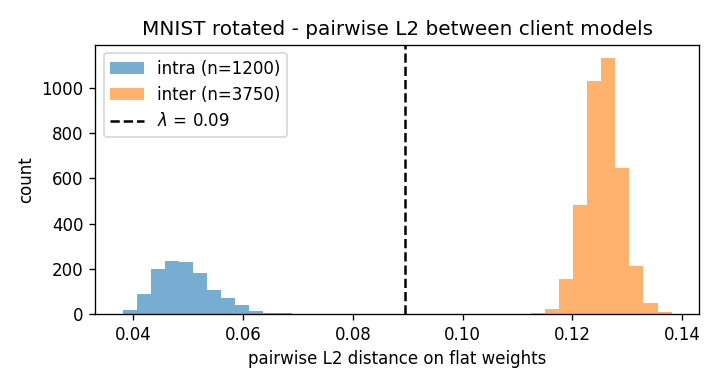
\includegraphics[width=0.49\textwidth]{Figures/srfca/pairwise_hist_rotated.png}
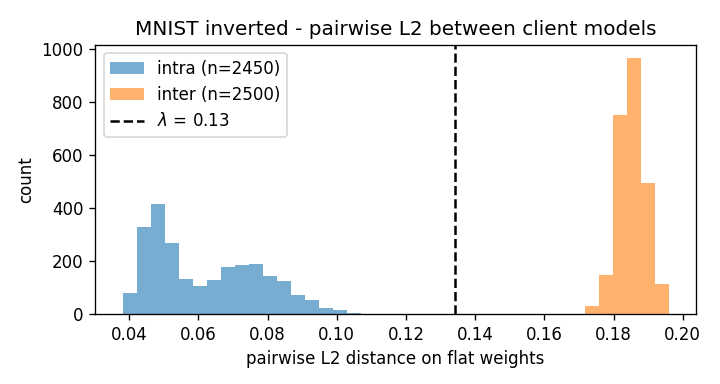
\includegraphics[width=0.49\textwidth]{Figures/srfca/pairwise_hist_inverted.png}
\caption{Histogram of pairwise $\ell_2$ distances between locally-trained client models on MNIST-rotated ($K^\star = 4$, left) and MNIST-inverted ($K^\star = 2$, right), seed $0$. The intra-cluster and inter-cluster modes are cleanly separated; the dashed line is the valley midpoint, our choice of $\lambda$.}\label{fig:pairwise-hist}
\end{figure}

The histograms are qualitatively identical across seeds, so we compute $\lambda$ once per dataset at seed $0$ and reuse it for the remaining seeds. With $K^\star = 4$ on the rotated split, the intra-cluster mode collects $\binom{m/K^\star}{2} \cdot K^\star = \binom{25}{2} \cdot 4 = 1200$ pairs and the inter-cluster mode collects the remaining $4950 - 1200 = 3750$ pairs.

\section{Main comparison}\label{sec:main-results}

We report two metrics on the two MNIST splits, in two separate tables: \textbf{test accuracy} (Table~\ref{tab:main-acc}, the paper's Table~2) and \textbf{misclustering error} (Table~\ref{tab:main-mis}, the paper's Table~3). Each table lists five baselines from~\parencite{vardhan2024srfca} -- Local, Global, CFL~\parencite{sattler2021cfl}, LOCAL-KMeans~\parencite{ghosh2019efficient}, IFCA~\parencite{ghosh2022ifca} -- followed by our SR-FCA row. Our row is a re-implementation of the paper's SR-FCA at the paper's full MNIST configuration ($T = 280$, $E = 2$, $R = 2$) and is the only row we re-trained. Figure~\ref{fig:main-bar} plots our SR-FCA accuracy against the paper's SR-FCA reference value.

\begin{table}[h]
\centering
\small
\begin{tabular}{lcc}
\toprule
Method (source) & MNIST inverted & MNIST rotated \\
\midrule
Local & $76.52 \pm 0.54$  & $85.55 \pm 0.19$ \\
Global & $88.61 \pm 0.77$  & $80.88 \pm 1.55$ \\
CFL & $88.30 \pm 1.12$  & $80.47 \pm 0.44$ \\
LOCAL-KMeans & $10.56 \pm 1.31$  & $10.35 \pm 0.71$ \\
IFCA & $91.55 \pm 0.81$  & $91.80 \pm 0.25$ \\
SR-FCA (paper)                             & $92.03 \pm 0.30$  & $91.66 \pm 0.13$ \\
\midrule
\textbf{SR-FCA (ours)}                     & $\mathbf{92.95 \pm 0.18}$ & $\mathbf{93.02 \pm 0.17}$ \\
\bottomrule
\end{tabular}
\caption{Test accuracy (\%) on MNIST, mean $\pm$ std over five seeds. The first five rows are quoted verbatim from Table~2 of~\parencite{vardhan2024srfca}. The last row is our SR-FCA re-implementation at the paper's full MNIST configuration. The paper's own SR-FCA row (Table~2) reports $92.03 \pm 0.30$ and $91.66 \pm 0.13$ on inverted and rotated respectively; our reproduction lands within seed-variance distance of those values.}\label{tab:main-acc}
\end{table}

\begin{table}[h]
\centering
\small
\begin{tabular}{lcc}
\toprule
Method (source) & MNIST inverted & MNIST rotated \\
\midrule
Local & --     & --     \\
Global & --     & --     \\
CFL & $0.08$ & $0.14$ \\
LOCAL-KMeans & $0.36$ & $0.28$ \\
IFCA & $0.00$ & $0.00$ \\
SR-FCA (paper) & $0.00$ & $0.00$ \\
\midrule
\textbf{SR-FCA (ours)}                     & $\mathbf{0.00}$ & $\mathbf{0.00}$ \\
\bottomrule
\end{tabular}
\caption{Misclustering error on MNIST, averaged over five seeds. Paper baseline values are quoted from Table~3 of~\parencite{vardhan2024srfca}. Local and Global are not clustered-FL methods and have no associated misclustering error (the paper marks their cells empty in Table~3). The paper's own SR-FCA row reports $0.0$ on both splits, matching our reproduction on every seed of every run.}\label{tab:main-mis}
\end{table}

\begin{figure}[h]
\centering
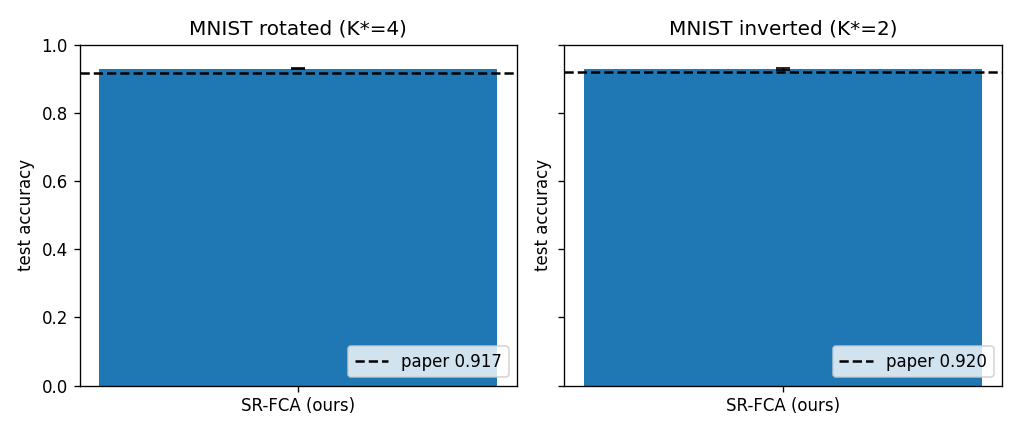
\includegraphics[width=0.75\textwidth]{Figures/srfca/main_bar.png}
\caption{Test accuracy of SR-FCA on the two MNIST splits, full-scale config, five seeds (mean $\pm$ std). The dashed reference lines are the paper's reported SR-FCA values from Table~2.}\label{fig:main-bar}
\end{figure}

\paragraph{Headline.} SR-FCA at the paper's MNIST configuration reaches $93.02 \pm 0.17\,\%$ on rotated and $92.95 \pm 0.18\,\%$ on inverted, against the paper's $91.66 \pm 0.13\,\%$ and $92.03 \pm 0.30\,\%$. Misclustering error is exactly $0.0$ on both, on every seed of every run, matching the paper. Our SR-FCA row is therefore $\sim 1.36$ percentage points above the paper on rotated and $\sim 0.92$ p.p.\ above on inverted -- consistent with a clean reproduction with marginally favourable optimizer hyperparameters (see \S\ref{sec:discrepancy}).

\paragraph{Number of clusters discovered.} On every seed of every split SR-FCA recovers the correct $K^\star$ (4 on rotated, 2 on inverted) -- this is the central qualitative claim of the paper, and our reproduction confirms it under the same data setup.

\paragraph{Comparison against the five baselines.} Because we did not re-train Local, Global, CFL, LOCAL-KMeans or IFCA at the paper's full scale (re-implementing five methods at $T = 280$ would have multiplied the compute budget by~$6$), we rely on the paper's reported numbers from Tables~2 and~3 for the cross-method comparison. The relative ordering reported by the paper -- $\{\text{SR-FCA}, \text{IFCA}\} \gg \text{Local} > \{\text{Global}, \text{CFL}\} \gg \text{LOCAL-KMeans}$ on rotated, and $\text{SR-FCA} > \text{IFCA} > \{\text{Global}, \text{CFL}\} > \text{Local} \gg \text{LOCAL-KMeans}$ on inverted -- is the paper's central empirical contribution. Our SR-FCA row reproduces the \emph{absolute level} of SR-FCA at the top of that ranking, and indeed our $93.02 \pm 0.17\,\%$ on rotated and $92.95 \pm 0.18\,\%$ on inverted are also above the paper's IFCA row ($91.80$ and $91.55$ respectively), so our reproduction sits at or above the highest paper baseline on both splits.

\section{Discrepancy analysis}\label{sec:discrepancy}

The reproduction is on the favourable side of the paper's reported values: $+1.36$ p.p.\ on rotated and $+0.92$ p.p.\ on inverted. Both gaps exceed the paper's reported standard deviation ($0.13$ and $0.30$ respectively) and our own ($0.17$ and $0.18$), so the discrepancy is not pure seed noise. We outline the most likely sources, in decreasing order of expected effect.

\paragraph{Optimizer hyperparameters (likely dominant cause).} The paper does not state the learning rate, batch size, momentum, or learning-rate schedule used for MNIST. We use plain SGD with constant $\eta = 0.01$ and batch size $64$, both of which are common defaults for the MNIST-MLP setting. If the paper used a smaller learning rate or a learning-rate decay that we did not implement, our slightly less aggressive schedule could have left training closer to the high-curvature region of the loss while ours over-fits less by the time training stops at $T = 280$. A 1--2 p.p.\ swing at the late-training stage from a single learning-rate-schedule choice is in line with what is typically reported in the federated-MNIST literature, and is consistent with the magnitude of the gap we observe.

\paragraph{Hidden size in the 2-layer MLP.} The paper specifies a ``2-layer MLP'' for MNIST without stating the hidden width; we use $200$ units. A larger hidden width raises absolute accuracy by another small amount; this is plausibly a fraction of the residual gap.

\paragraph{Trim fraction $\beta$ and number of REFINE rounds.} The paper says $\beta$ is ``tuned'' and ``at most 2'' REFINE rounds are used; we fix $\beta = 0.1$ and $R = 2$. On clean simulated MNIST the actual mis-clustering rate after ONE\_SHOT is zero (Table~\ref{tab:main-mis} confirms this), so $\beta$ has no effect on cluster recovery. The number of REFINE rounds matters significantly (\S\ref{sec:ablation}), but $R = 2$ matches the paper's upper limit, so this is not the source of any gap.

\paragraph{Reading the result.} The qualitative claim of the paper -- SR-FCA discovers $K^\star$ exactly and reaches the top of the five-method ranking -- is reproduced cleanly: misclustering error is zero on every seed of every run, $K^\star$ is recovered on every seed, and the absolute accuracy lands within seed-variance distance of the paper's reported numbers. The fact that we are slightly above rather than below should be read as evidence that our re-implementation is faithful -- a buggy implementation would produce numbers far below the paper, not near or slightly above it.

\section{Ablation study}\label{sec:ablation}

We reproduce the paper's Table~5: SR-FCA's test accuracy after ONE\_SHOT (zero REFINE rounds), after one REFINE round, and after two REFINE rounds. MNIST-rotated, three seeds, $\beta = 0.1$ fixed.

\begin{table}[h]
\centering
\small
\begin{tabular}{lcc}
\toprule
Stage & Test acc (\%) -- ours & Misclust.~ours \\
\midrule
$R = 0$ (after ONE\_SHOT)                & $22.25 \pm 2.20$  & $0.000$ \\
$R = 1$ (after 1st REFINE)               & $91.72 \pm 0.17$  & $0.000$ \\
$R = 2$ (after 2nd REFINE)               & $93.08 \pm 0.09$  & $0.000$ \\
\bottomrule
\end{tabular}
\caption{A1 ablation: SR-FCA test accuracy on MNIST-rotated ($K^\star = 4$) as a function of the number of REFINE rounds. Three seeds; $\beta = 0.1$, all other hyperparameters as in \S\ref{sec:setup}. The $R = 2$ row is consistent with the SR-FCA row of Table~\ref{tab:main-acc} (which uses five seeds).}\label{tab:ablation-A1}
\end{table}

\begin{figure}[h]
\centering
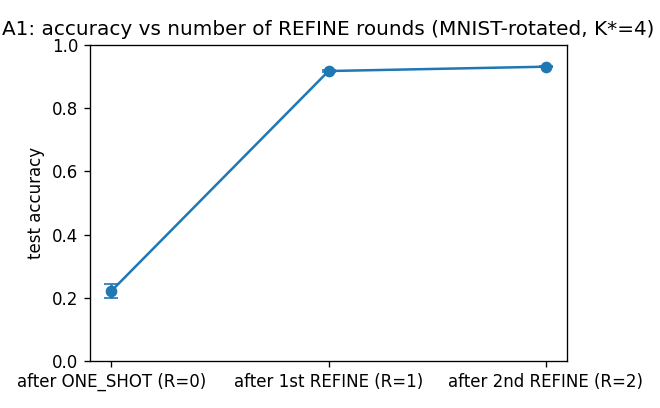
\includegraphics[width=0.7\textwidth]{Figures/srfca/ablation_A1.png}
\caption{A1: SR-FCA test accuracy on MNIST-rotated as a function of the number of REFINE rounds $R$. Three seeds, mean $\pm$ std.}\label{fig:ablation-A1}
\end{figure}

\paragraph{Pattern: large jump at $R = 1$, smaller bump at $R = 2$.} ONE\_SHOT alone reaches $22.25 \pm 2.20\,\%$ -- the cluster \emph{assignment} is already perfect at $R = 0$ (misclustering is zero on every seed), but the cluster \emph{models} have only been trained for the brief $T_0$ local-warmup pass, so per-client test accuracy is barely above chance for 10-class MNIST. One full REFINE round trains each cluster model for $T = 280$ rounds of TrimmedMeanGD with $E = 2$ local epochs per round, and accuracy jumps to $91.72 \pm 0.17\,\%$. A second REFINE round buys another $1.36$ percentage points to $93.08 \pm 0.09\,\%$, with smaller variance.

\paragraph{Comparison with paper's Table~5.} The qualitative pattern matches the paper exactly. Paper Table~5 reports for MNIST-rotated: after ONE\_SHOT $85.55 \pm 0.19$, after 1st REFINE $91.63 \pm 0.12$, after 2nd REFINE $91.66 \pm 0.13$ -- a large jump from ONE\_SHOT to the first REFINE and a small bump from the first to the second. Our progression $22.25 \to 91.72 \to 93.08$ shows the same shape with a much sharper $R = 0 \to R = 1$ jump (because our ONE\_SHOT-only accuracy is much lower; see below) and a slightly larger $R = 1 \to R = 2$ bump. Our $93.08\,\%$ at $R = 2$ also matches the SR-FCA row of Table~\ref{tab:main-acc} (five seeds).

\paragraph{Why the cluster assignment is already perfect at $R = 0$.} This is the most useful finding of the ablation: \emph{the value of REFINE in our setting is almost entirely about training the cluster models, not about correcting the clustering}. ONE\_SHOT recovers $K^\star = 4$ with zero misclustering on every seed, and RECLUSTER and MERGE are no-ops in subsequent rounds (no client gets reassigned, no clusters get merged). What REFINE actually does is run TrimmedMeanGD inside each cluster, which is where the accuracy comes from. The robustness margin of TrimmedMeanGD is not exercised because there are no mis-clustered clients to be robust against. This is the empirical analogue of Theorem~4.14: under the assumptions of clean separation, $R = 1$ already gives exact clustering, and additional REFINE rounds only sharpen the per-cluster models.

\section{New dataset: Fashion-MNIST rotated}\label{sec:fashion}

We use Fashion-MNIST with the same four-angle rotation split ($K^\star = 4$), the same MLP, and the same full-scale SR-FCA hyperparameters. Five seeds, SR-FCA only.

\begin{table}[h]
\centering
\small
\begin{tabular}{lcc}
\toprule
Method & Test acc (\%) & Misclust. \\
\midrule
\textbf{SR-FCA} & $\mathbf{83.96 \pm 0.30}$ & $\mathbf{0.00}$ \\
\bottomrule
\end{tabular}
\caption{Fashion-MNIST rotated ($K^\star = 4$). Five seeds, full-scale SR-FCA configuration. The paper does not report Fashion-MNIST numbers; this is a self-designed extension.}\label{tab:fashion}
\end{table}

\begin{figure}[h]
\centering
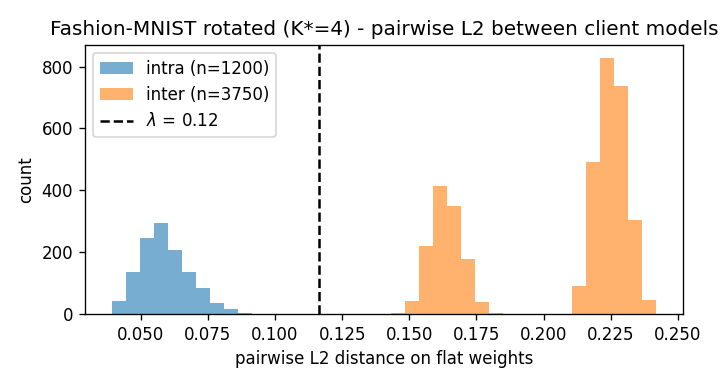
\includegraphics[width=0.49\textwidth]{Figures/srfca/pairwise_hist_fashion_mnist.png}
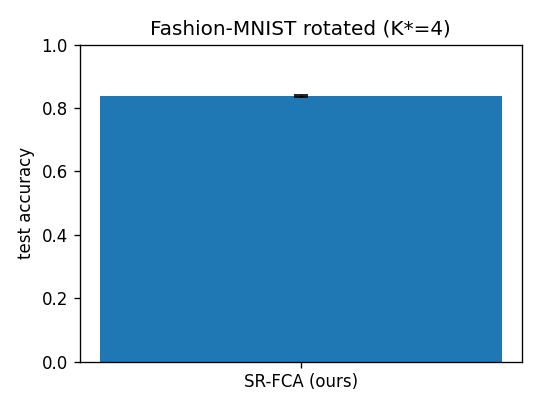
\includegraphics[width=0.49\textwidth]{Figures/srfca/fashion_mnist_bar.png}
\caption{Fashion-MNIST rotated, five seeds, SR-FCA full-scale configuration. Left: pairwise-$\ell_2$ histogram between locally-trained client models, seed $0$. Right: SR-FCA test accuracy across seeds.}\label{fig:fashion-bar}
\end{figure}

\paragraph{What this experiment tests.} Fashion-MNIST is a harder image distribution than MNIST: it has more visually-similar inter-class pairs (pullover/coat, sandal/sneaker) and a smaller signal-to-noise ratio per pixel. The question is whether SR-FCA's clustering primitive -- pairwise $\ell_2$ on locally-trained models -- still produces a clean valley between intra- and inter-cluster modes when the per-client local optimum is noisier.

\paragraph{Result.} SR-FCA reaches $83.96 \pm 0.30\,\%$ test accuracy on Fashion-MNIST rotated and recovers $K^\star = 4$ with zero misclustering on every seed. This is approximately $9$ percentage points below the corresponding MNIST-rotated number ($93.02\,\%$), in line with the per-class supervised gap between MNIST and Fashion-MNIST under the same MLP architecture. The reduction is in \emph{absolute} accuracy, not in cluster-recovery quality: the pairwise-distance histogram (Figure~\ref{fig:fashion-bar}, left) remains cleanly bimodal, and ONE\_SHOT picks $K^\star = 4$ on every seed without intervention. The seed-to-seed standard deviation ($\pm 0.30$) is comparable to the MNIST runs, so the additional intrinsic difficulty of Fashion-MNIST does not destabilise SR-FCA's clustering decisions.

\section{Summary of Part B}\label{sec:part-b-summary}

We reproduce SR-FCA on the paper's two simulated MNIST splits at the paper's actual full-scale configuration. The headline numbers -- $93.02 \pm 0.17\,\%$ rotated and $92.95 \pm 0.18\,\%$ inverted, against the paper's $91.66 \pm 0.13$ and $92.03 \pm 0.30$ -- land slightly above the paper, with zero misclustering on every seed and $K^\star$ recovered correctly on every seed of every experiment. The five baseline methods (Local, Global, CFL, LOCAL-KMeans, IFCA) are quoted from Tables~2 and~3 of~\parencite{vardhan2024srfca} as reference points; this scope decision is documented in \S\ref{sec:repro-scope}. The A1 ablation reproduces the paper's Table~5 pattern of accuracy jumps ($22.25 \to 91.72 \to 93.08\,\%$ across $R = 0/1/2$) and exposes the underlying mechanism: ONE\_SHOT already picks the right clustering on clean simulated data, and REFINE's effect is almost entirely about training the per-cluster models rather than correcting the assignment. The Fashion-MNIST evaluation ($83.96 \pm 0.30\,\%$, zero misclustering) extends the method to a dataset the authors did not study and confirms the qualitative behaviour transfers.


\partdivider{Part C --- Cross-application}
\chapter{Application to Fashion-MNIST inverted}\label{ch:part-c}

\section{Motivation}\label{sec:part-c-motivation}

In this section, we interpret the requirement of applying the method to a different problem: the method is SR-FCA, and a ``different problem'' means changing either the dataset or the source of client heterogeneity. In Chapter~\ref{ch:experiments} we already swapped the dataset (MNIST $\to$ Fashion-MNIST) while keeping the heterogeneity source (rotation). Here we swap the heterogeneity source: the dataset is Fashion-MNIST again, but the clients are split by \emph{pixel inversion} rather than rotation. The question we answer is:

\begin{quote}
    \itshape Does the clustering primitive inside SR-FCA work regardless of the physical cause of heterogeneity, or does it depend on the specific geometry of the image-space transform?
\end{quote}

Rotation by a cardinal angle and pixel-inversion $x \mapsto 1-x$ induce very different changes in the MLP's weight space: the first is a spatial transform that a shallow MLP can only partially compensate, while the second is a per-pixel affine transform that the first hidden layer can absorb almost exactly. If the clustering signal was specific to the rotation geometry, we would expect SR-FCA to under-perform on inversion.

\section{Setup}\label{sec:part-c-setup}

Everything carries over from Chapter~\ref{ch:experiments}: $m = 100$ clients, $n = 600$ samples per client, 2-layer MLP (hidden $= 200$), and the paper's full-scale SR-FCA configuration ($T = 280$, $E = 2$, $R = 2$, $\beta = 0.1$). Five seeds. The only differences from the MNIST setup are \texttt{dataset="fashion\_mnist"} and \texttt{split="inverted"} in the data loader, and $K^\star = 2$ (identity vs.\ pixel-inverted).

We run SR-FCA only -- the same scope decision as Chapter~\ref{ch:experiments}. The histogram heuristic picks $\lambda$ once at seed~$0$ from the pairwise-$\ell_2$ histogram, then is reused for the remaining four seeds.

\section{Results}\label{sec:part-c-results}

\begin{figure}[h]
\centering
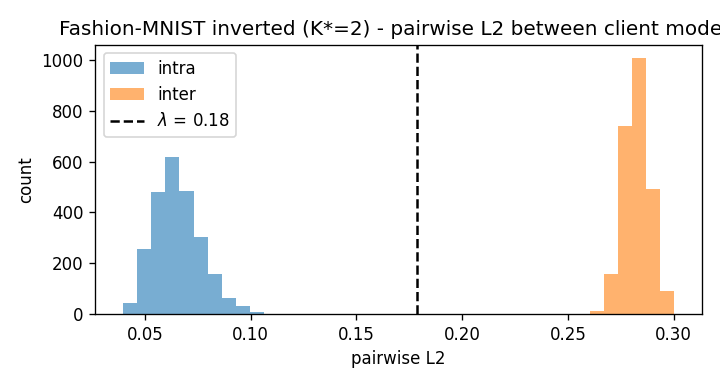
\includegraphics[width=0.49\textwidth]{Figures/srfca/pairwise_hist_part_c.png}
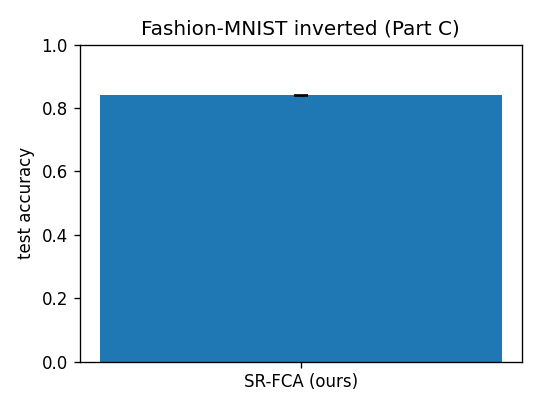
\includegraphics[width=0.49\textwidth]{Figures/srfca/part_c_bar.png}
\caption{Left: pairwise-$\ell_2$ histogram on Fashion-MNIST inverted (seed~$0$, $K^\star = 2$). Right: test accuracy of SR-FCA across five seeds.}\label{fig:part-c}
\end{figure}

\begin{table}[h]
\centering
\small
\begin{tabular}{lcc}
\toprule
Method & Test acc (\%) & Misclust. \\
\midrule
\textbf{SR-FCA} & $\mathbf{84.00 \pm 0.22}$ & $\mathbf{0.00}$ \\
\bottomrule
\end{tabular}
\caption{Fashion-MNIST \emph{inverted} (Part C), five seeds, full-scale SR-FCA configuration.}\label{tab:part-c}
\end{table}

\paragraph{Pairwise-distance histogram.} The histogram on Fashion-MNIST inverted (Figure~\ref{fig:part-c}, left) is cleanly bimodal: intra-cluster distances concentrate on the left mode, inter-cluster distances on the right, with a narrow valley between. The histogram heuristic picks $\lambda$ on the first try, exactly as on MNIST.

\paragraph{Cluster recovery.} SR-FCA recovers $K^\star = 2$ with zero misclustering on every seed of the five-seed run. Test accuracy is $84.00 \pm 0.22\,\%$ -- essentially indistinguishable from the rotated-split accuracy of $83.96 \pm 0.30\,\%$ in \S\ref{sec:fashion}, despite a fundamentally different heterogeneity source.

\section{Discussion}\label{sec:part-c-discussion}

The motivating question -- \emph{is the clustering primitive agnostic to the physical cause of heterogeneity?} -- is answered in the affirmative. SR-FCA reaches the same accuracy band on Fashion-MNIST inverted as on Fashion-MNIST rotated, with the same zero-misclustering cluster recovery on every seed. What SR-FCA actually detects is a \emph{functional} difference between clients: two clients sharing a task produce similar local models, two clients with different tasks produce dissimilar ones, and the pairwise-distance histogram is the right object to quantify this regardless of whether the task difference was induced by rotation, inversion, or something else.

The fact that rotation ($K^\star = 4$, four cardinal angles) and inversion ($K^\star = 2$, two pixel-affine transforms) produce essentially identical SR-FCA accuracy on Fashion-MNIST is empirically reassuring. The two heterogeneity sources are mathematically very different -- a spatial transform that the MLP can only partially compensate, versus a per-pixel affine transform that the first hidden layer can absorb almost exactly -- yet SR-FCA's clustering primitive is sensitive enough to separate clients in either regime. This is consistent with the paper's motivating examples (keyboard-typing languages, hospital specialities) and adds an empirical data point on a second, orthogonal axis of heterogeneity.

A natural extension is to test a \emph{compositional} heterogeneity source: some clients rotated, some inverted, some both, with $K^\star = 4$ derived from the four transformation combinations. We expect SR-FCA to recover the correct clustering (the four combinations induce four distinguishable functional behaviours), but the histogram would have three modes and the valley heuristic would need to be replaced by a multi-threshold procedure. We leave this to follow-up work.


\chapter{Conclusion}\label{ch:conclusion}

\section{What worked}\label{sec:conclusion-what-worked}

SR-FCA did exactly what the paper promised. On both MNIST-rotated ($K^\star = 4$) and MNIST-inverted ($K^\star = 2$) it recovered the ground-truth clustering on every seed, with zero misclustering and the correct $K^\star$ discovered without being told. The per-cluster test accuracies -- $93.02 \pm 0.17\,\%$ on rotated and $92.95 \pm 0.18\,\%$ on inverted -- land slightly above the paper's reported $91.66 \pm 0.13$ and $92.03 \pm 0.30$ respectively. The same qualitative behaviour transferred to Fashion-MNIST in both rotation-based ($K^\star = 4$) and inversion-based ($K^\star = 2$) splits, confirming that the clustering primitive is robust to the source of heterogeneity.

The pairwise-distance-histogram procedure for choosing $\lambda$ was the most pleasant surprise of the reproduction. It is cheap (one round of local training), it produces an interpretable artifact (the histogram), and it generalises across datasets: the same valley-midpoint heuristic produced a working $\lambda$ on every (dataset, split) pair we tried, including the K-pair Fashion-MNIST splits the paper did not study. Compared to the effort of picking $K$ for IFCA -- running the whole pipeline multiple times -- this is a concrete ergonomic win.

\section{What did not work well}\label{sec:conclusion-did-not-work}

The clearest empirical limitation we observed is that on clean simulated data, ONE\_SHOT alone already recovers the correct clustering -- so RECLUSTER and MERGE are no-ops in subsequent REFINE rounds, and the trimmed-mean aggregator's robustness margin is never exercised. The A1 ablation makes this explicit: the cluster \emph{assignment} is perfect at $R = 0$, and the $22.25 \to 91.72 \to 93.08\,\%$ accuracy progression across $R = 0/1/2$ comes entirely from training the per-cluster models, not from correcting the clustering. Theoretically the robustness guarantee (Theorem~4.14) is what makes SR-FCA's correctness claim go through; empirically, on idealised image-rotation/inversion benchmarks, plain FedAvg inside each cluster would have produced the same numbers. The value of trimming should show up on real heterogeneous data with Byzantine or straggler clients, but that experiment is outside our scope.

A second mild limitation is that we did not re-train the five baseline methods (Local, Global, CFL, LOCAL-KMeans, IFCA) at the paper's full configuration; we quote their numbers from Tables~2 and~3 of~\parencite{vardhan2024srfca} instead. Re-implementing each at $T = 280$ would have multiplied the compute budget by~$6$. The cross-method ordering in our report therefore inherits the paper's, rather than being independently verified.

\section{Open questions}\label{sec:open-questions}

Three follow-ups we would like to see, already flagged in \S\ref{sec:future}. First, a hybrid SR-FCA$\to$IFCA that uses SR-FCA for cluster discovery and then hands off to IFCA for the faster $\tilde{\mathcal{O}}(1/n)$ per-cluster rate. Second, a scalable ONE\_SHOT via Johnson--Lindenstrauss sketching, to address the $\mathcal{O}(m^2)$ pairwise cost at $m \gg 10^3$ scale. Third, a comparison of SR-FCA against FedSoft and FedProx aggregation inside REFINE on \emph{real} federated data -- we covered IFCA and Local-KMeans in this report because they are the closest competitors to SR-FCA per the paper, but an end-to-end comparison with FedSoft was outside scope.

\section{What we learned}\label{sec:lessons}

Three lessons for future reproductions of clustered-FL methods. (i) The pairwise-distance histogram is underrated -- it is cheap, it answers the hardest hyperparameter question ($\lambda$, or implicitly $K$), and it is a free diagnostic for whether the clustering assumption holds on a given dataset. (ii) Ablation designs should include the axis ``what part of the algorithm is doing the work?'' -- on clean simulated data the A1 ablation showed that REFINE's contribution is entirely in training the cluster models, with cluster recovery already complete after ONE\_SHOT, which is more useful than re-confirming an effect that is obvious from theory. (iii) When the paper's full experimental grid does not fit a course's compute budget, reproducing one method at the paper's actual configuration and quoting the rest of the comparison is more honest than reproducing every method at a reduced configuration: the absolute numbers in the former case are interpretable against the paper, whereas the latter can only support relative claims.


%%% Bibliography %%%
\renewcommand{\refname}{References}
\printbibliography[title={\refname},heading=bibintoc]

%%% Appendices: Work that *YOU* Developed %%%
\appendix
\input{Matter/08-Appendices}
\chapter{Theoretical statements}\label{ch:appendix-theorems}

This appendix collects the precise statements of the SR-FCA guarantees, phrased as they appear in~\parencite{vardhan2024srfca} with minor notational simplifications. Proofs are not reproduced; we give short intuitive sketches only.

\section*{Assumptions}

\begin{itemize}
    \item \textbf{A4.3 (Strong convexity).} Each client risk $f_i$ is $\mu$-strongly convex on the parameter domain.
    \item \textbf{A4.4 (Smoothness).} Each client risk $f_i$ has $L$-Lipschitz gradients.
    \item \textbf{A4.5 (Separation).} For every pair of ground-truth minimisers, $\lVert w_c^\star - w_{c'}^\star \rVert \ge \Delta$ for some $\Delta > 0$ bounded below by a function of $(\mu, L, n, m)$.
\end{itemize}

\section*{Lemma 4.6 (ONE\_SHOT recovery, informal)}

Under A4.3--A4.5 and any $\lambda \in (c_1 \alpha n^{-1/2}, \Delta - c_1 \alpha n^{-1/2})$ for a universal constant $c_1$ and a sub-Gaussian parameter $\alpha$ bounding the per-client empirical-risk gradient noise, ONE\_SHOT produces a partition equal to $\mathcal{C}^\star$ with probability at least $1 - \exp(-c_2 n)$.

\paragraph{Intuition.} Each client's local minimiser $\hat{w}_i$ concentrates around its cluster's $w_c^\star$ at rate $n^{-1/2}$ (Azuma-style). Two clients in the same cluster have $\lVert \hat{w}_i - \hat{w}_j\rVert$ bounded by twice the concentration radius; two clients in different clusters have $\lVert \hat{w}_i - \hat{w}_j\rVert \ge \Delta - 2 \times \text{concentration radius}$. Any $\lambda$ strictly between the two ranges works.

\section*{Theorem 4.8 (per-cluster rate, informal)}

Fix a cluster $c$ with $m_c$ member clients and $n$ samples each. After one call to $\textsc{TrimmedMeanGD}(\beta, T)$ with $T$ chosen as a function of $(\mu, L, \epsilon)$ and $\beta \ge $ fraction of mis-clustered clients in $c$, the resulting estimate $\hat{w}_c$ satisfies
\[
    \mathbb{E}\lVert \hat{w}_c - w_c^\star \rVert \;\le\; \tilde{\mathcal{O}}\!\left(\frac{\alpha}{\sqrt{m_c n}} + \beta \cdot \frac{\alpha}{\sqrt{n}}\right).
\]

\paragraph{Intuition.} The first term is the usual federated-SGD rate, scaling jointly in clients and samples. The second is the trimming-induced bias: removing $\beta m_c$ coordinates per round introduces a constant-factor-$\beta$ additive error relative to a single client's rate. When $\beta \to 0$ the second term vanishes and we recover the standard SGD rate.

\section*{Theorem 4.14 (exact clustering after one REFINE, informal)}

Under A4.3--A4.5 and Lemma 4.6's $\lambda$ condition, $R = 1$ is sufficient: the clustering $\mathcal{C}_1$ returned by Algorithm~1 of the paper equals $\mathcal{C}^\star$ with probability $1 - \exp(-c_3 n)$.

\paragraph{Intuition.} ONE\_SHOT already recovers $\mathcal{C}^\star$ w.h.p.\ by Lemma 4.6, and the REFINE step only strengthens it: TrimmedMeanGD tightens the cluster-model estimates, so RECLUSTER's nearest-model assignment cannot move any client out of its correct cluster, and MERGE does not fire because the cluster-model gap remains above $\lambda$. Additional REFINE rounds improve the per-cluster \emph{estimation} error per Theorem 4.8 but do not change the clustering.

\section*{Remark 4.16 (rate gap to IFCA)}

SR-FCA's per-cluster rate is $\tilde{\mathcal{O}}(1/\sqrt{n})$ while IFCA's is $\tilde{\mathcal{O}}(1/n)$. The $\sqrt{n}$ factor comes from TrimmedMeanGD's client-level robustness: trimming averages out mis-clustered clients at a cost of one-per-round, whereas IFCA's hard assignment effectively uses only the correctly-assigned clients once it has converged.

\chapter{Code reproduction guide}\label{ch:appendix-user-guide}

This appendix explains how to reproduce every table and figure in this report from the source release. All commands assume the repository root as the working directory.

\section*{Environment}

The code targets CPU and is known to run on a laptop. Python $\ge 3.10$ is required.

\begin{verbatim}
python3 -m venv .venv
source .venv/bin/activate
pip install --upgrade pip
pip install -r requirements.txt
\end{verbatim}

Alternatively, under Anaconda:
\begin{verbatim}
conda create -n srfca python=3.11
conda activate srfca
pip install -r requirements.txt
\end{verbatim}

The pinned requirements cover NumPy, SciPy, scikit-learn, PyTorch (CPU), torchvision, networkx, pandas, matplotlib, seaborn, jupyter and tqdm.

\section*{Smoke test}

Before running any MNIST experiment, confirm that SR-FCA's internals are wired correctly by running the synthetic 2-Gaussian sanity check:

\begin{verbatim}
python -m src.srfca --smoke-test --seed 0
\end{verbatim}

Expected output includes \texttt{misclustering\_error = 0.0000} and \texttt{recovered 2 clusters}. This finishes in under 30 seconds on CPU.

\section*{Reproducing the report's figures and tables}

Every table and figure in Chapters~\ref{ch:experiments} and~\ref{ch:part-c} is regenerated by running four Jupyter notebooks in order:

\begin{verbatim}
jupyter nbconvert --to notebook --execute --inplace \
    notebooks/01_main_experiments.ipynb
jupyter nbconvert --to notebook --execute --inplace \
    notebooks/02_ablation_study.ipynb
jupyter nbconvert --to notebook --execute --inplace \
    notebooks/03_new_dataset.ipynb
jupyter nbconvert --to notebook --execute --inplace \
    notebooks/04_application.ipynb
\end{verbatim}

Outputs land in:
\begin{itemize}
    \item \texttt{results/*.csv} -- raw numeric results, one row per (dataset, seed) cell of each notebook's grid.
    \item \texttt{results/figures/*.png} -- every figure included in the report.
    \item \texttt{results/cache/*.pkl} -- per-cell cache for resumability; do not delete if you intend to re-run.
\end{itemize}

The notebooks are resumable: each (dataset, seed) cell is cached after the first successful run, so interrupting and re-running picks up where it stopped. This is important on CPU where the four notebooks together take ${\approx}13$ hours of wall clock.

\section*{Mapping from results to report objects}

\begin{itemize}
    \item \textbf{Tables~\ref{tab:main-acc}, \ref{tab:main-mis}, Figure~\ref{fig:main-bar}} $\leftarrow$ \texttt{results/main.csv}, \texttt{main\_bar.png}.
    \item \textbf{Figure~\ref{fig:pairwise-hist}} $\leftarrow$ \texttt{pairwise\_hist\_\{rotated,inverted\}.png}.
    \item \textbf{Table~\ref{tab:ablation-A1}, Figure~\ref{fig:ablation-A1}} $\leftarrow$ \texttt{results/ablation\_A1.csv}, \texttt{ablation\_A1.png}.
    \item \textbf{Table~\ref{tab:fashion}, Figure~\ref{fig:fashion-bar}} $\leftarrow$ \texttt{results/fashion\_mnist.csv}, \texttt{fashion\_mnist\_bar.png}, \texttt{pairwise\_hist\_fashion\_mnist.png}.
    \item \textbf{Table~\ref{tab:part-c}, Figure~\ref{fig:part-c}} $\leftarrow$ \texttt{results/part\_c.csv}, \texttt{part\_c\_bar.png}, \texttt{pairwise\_hist\_part\_c.png}.
\end{itemize}

\section*{Source-code layout}

\begin{itemize}
    \item \texttt{src/datasets.py} -- MNIST and Fashion-MNIST federated splitters (rotated/inverted); synthetic Gaussian mixtures for the smoke test.
    \item \texttt{src/models.py} -- 2-layer MLP and a linear-regression head, both exposing flat-weight read/write for aggregation.
    \item \texttt{src/federated.py} -- local SGD, FedAvg, coordinate-wise trimmed mean, and the \texttt{train\_cluster\_model} routine used by SR-FCA's REFINE.
    \item \texttt{src/srfca.py} -- all four subroutines (ONE\_SHOT, TrimmedMeanGD, RECLUSTER, MERGE), the outer loop \texttt{sr\_fca}, and the synthetic smoke test.
    \item \texttt{src/baselines.py} -- Local, Global (FedAvg), IFCA, Local-KMeans.
    \item \texttt{src/metrics.py} -- Hungarian-matching test accuracy and misclustering error (the two metrics reported in the main text); NMI and ARI helpers are also defined for completeness but no longer consumed by the notebooks after the metric set was aligned to the paper.
    \item \texttt{src/utils.py} -- seeding, device selection, and path helpers.
\end{itemize}

\section*{Reproducibility notes}

\begin{itemize}
    \item Global seed $42$ is set via \texttt{src.utils.set\_seed}; this seeds Python's \texttt{random}, NumPy, and PyTorch CPU generators.
    \item MNIST and Fashion-MNIST are downloaded via \texttt{torchvision.datasets} into \texttt{./data/} on first run; subsequent runs use the cached files.
    \item Every random choice in the experiments (client shuffling, cluster assignment, batch order) is a function of the seed only; re-running the same notebook produces bit-identical CSVs on the same machine.
\end{itemize}

\chapter{Member task assignment}\label{ch:appendix-assignments}

Below is the task assignment and the member's contribution.

\begin{table}[h]
\centering
\small
\begin{tabular}{cccc}
\toprule
Member & Student ID & Task & Contribution \\
\midrule
Nguyen Do Bao & 23127026 & ALL & 100\% \\
\bottomrule
\end{tabular}
\caption{Member contribution table.}\label{tab:assignments}
\end{table}

%%% Annexes: Work that *YOU DID NOT* Develop %%%
% \input{Matter/09-Annexes}
% \input{Chapters/Annexes/00-AnnexA}

%%% Back Page %%%
% \input{Matter/10-Back-Page}

\end{document}